% Conceptual flow chart of the MD-LDP for the presentation (no equations, no parameter values).
% Detailed version: MD_LDP_v1.tex. Compile: pdflatex MD_LDP_concept.tex
\documentclass[tikz, border=4pt]{standalone}
\usepackage[scaled]{helvet}
\renewcommand{\familydefault}{\sfdefault}
\usetikzlibrary{positioning, arrows.meta, calc}

\definecolor{shared}{HTML}{4A5568}
\definecolor{dOne}{HTML}{1F77B4}
\definecolor{dTwo}{HTML}{D95F02}

\tikzset{
    box/.style    = {draw=shared, line width=0.8pt, rounded corners=3pt, fill=shared!6, align=center,
                     font=\small, inner sep=4pt, text width=#1, minimum height=11mm},
    box/.default  = 3.3cm,
    out/.style    = {draw=#1, line width=1.1pt, rounded corners=3pt, fill=#1!12, align=center,
                     font=\small, inner sep=4pt, text width=3.6cm, minimum height=11mm},
    arrow/.style  = {-{Stealth[length=2mm]}, line width=0.8pt, draw=shared},
}

\begin{document}
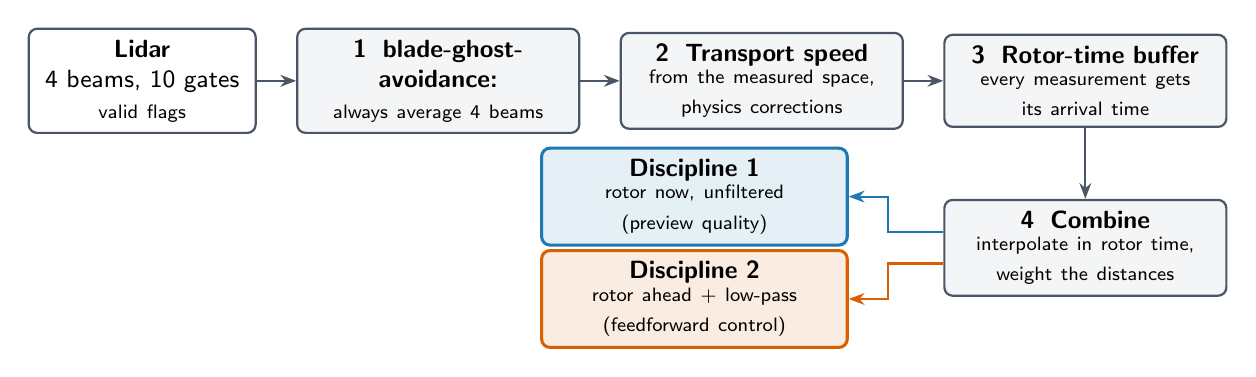
\begin{tikzpicture}[node distance=5mm]
\node[box=2.6cm, fill=white]   (in)  {\textbf{Lidar}\\ 4 beams, 10 gates\\ \scriptsize valid flags};
\node[box, right=of in]        (cs)  {\textbf{1\; blade-ghost-avoidance:}\\ \scriptsize always average 4 beams};
\node[box, right=of cs]        (sp)  {\textbf{2\; Transport speed}\\ \scriptsize from the measured space,\\ physics corrections};
\node[box, right=of sp]        (rt)  {\textbf{3\; Rotor-time buffer}\\ \scriptsize every measurement gets\\ its arrival time};
\node[box, below=9mm of rt]    (cb)  {\textbf{4\; Combine}\\ \scriptsize interpolate in rotor time,\\ weight the distances};
\node[out=dOne, left=12mm of cb, yshift=6.5mm] (d1)
    {\textbf{Discipline 1}\\ \scriptsize rotor now, unfiltered\\ (preview quality)};
\node[out=dTwo, left=12mm of cb, yshift=-6.5mm] (d2)
    {\textbf{Discipline 2}\\ \scriptsize rotor ahead + low-pass\\ (feedforward control)};

\draw[arrow] (in) -- (cs);
\draw[arrow] (cs) -- (sp);
\draw[arrow] (sp) -- (rt);
\draw[arrow] (rt) -- (cb);
\draw[arrow, draw=dOne] ($(cb.west) + (0, 2mm)$) -| ($(d1.east) + (5mm, 0)$) -- (d1.east);
\draw[arrow, draw=dTwo] ($(cb.west) + (0, -2mm)$) -| ($(d2.east) + (5mm, 0)$) -- (d2.east);
\end{tikzpicture}
\end{document}
